\section{Background}
\label{sec:background}
This section provides the necessary background of the blockchain execution environment. We briefly introduce the core execution model of the Ethereum Virtual Machine (EVM), its resource metering mechanism known as Gas, and the distinct node workloads that motivate the dual-mode design of Helios.

\begin{figure}[!htbp]
\centering
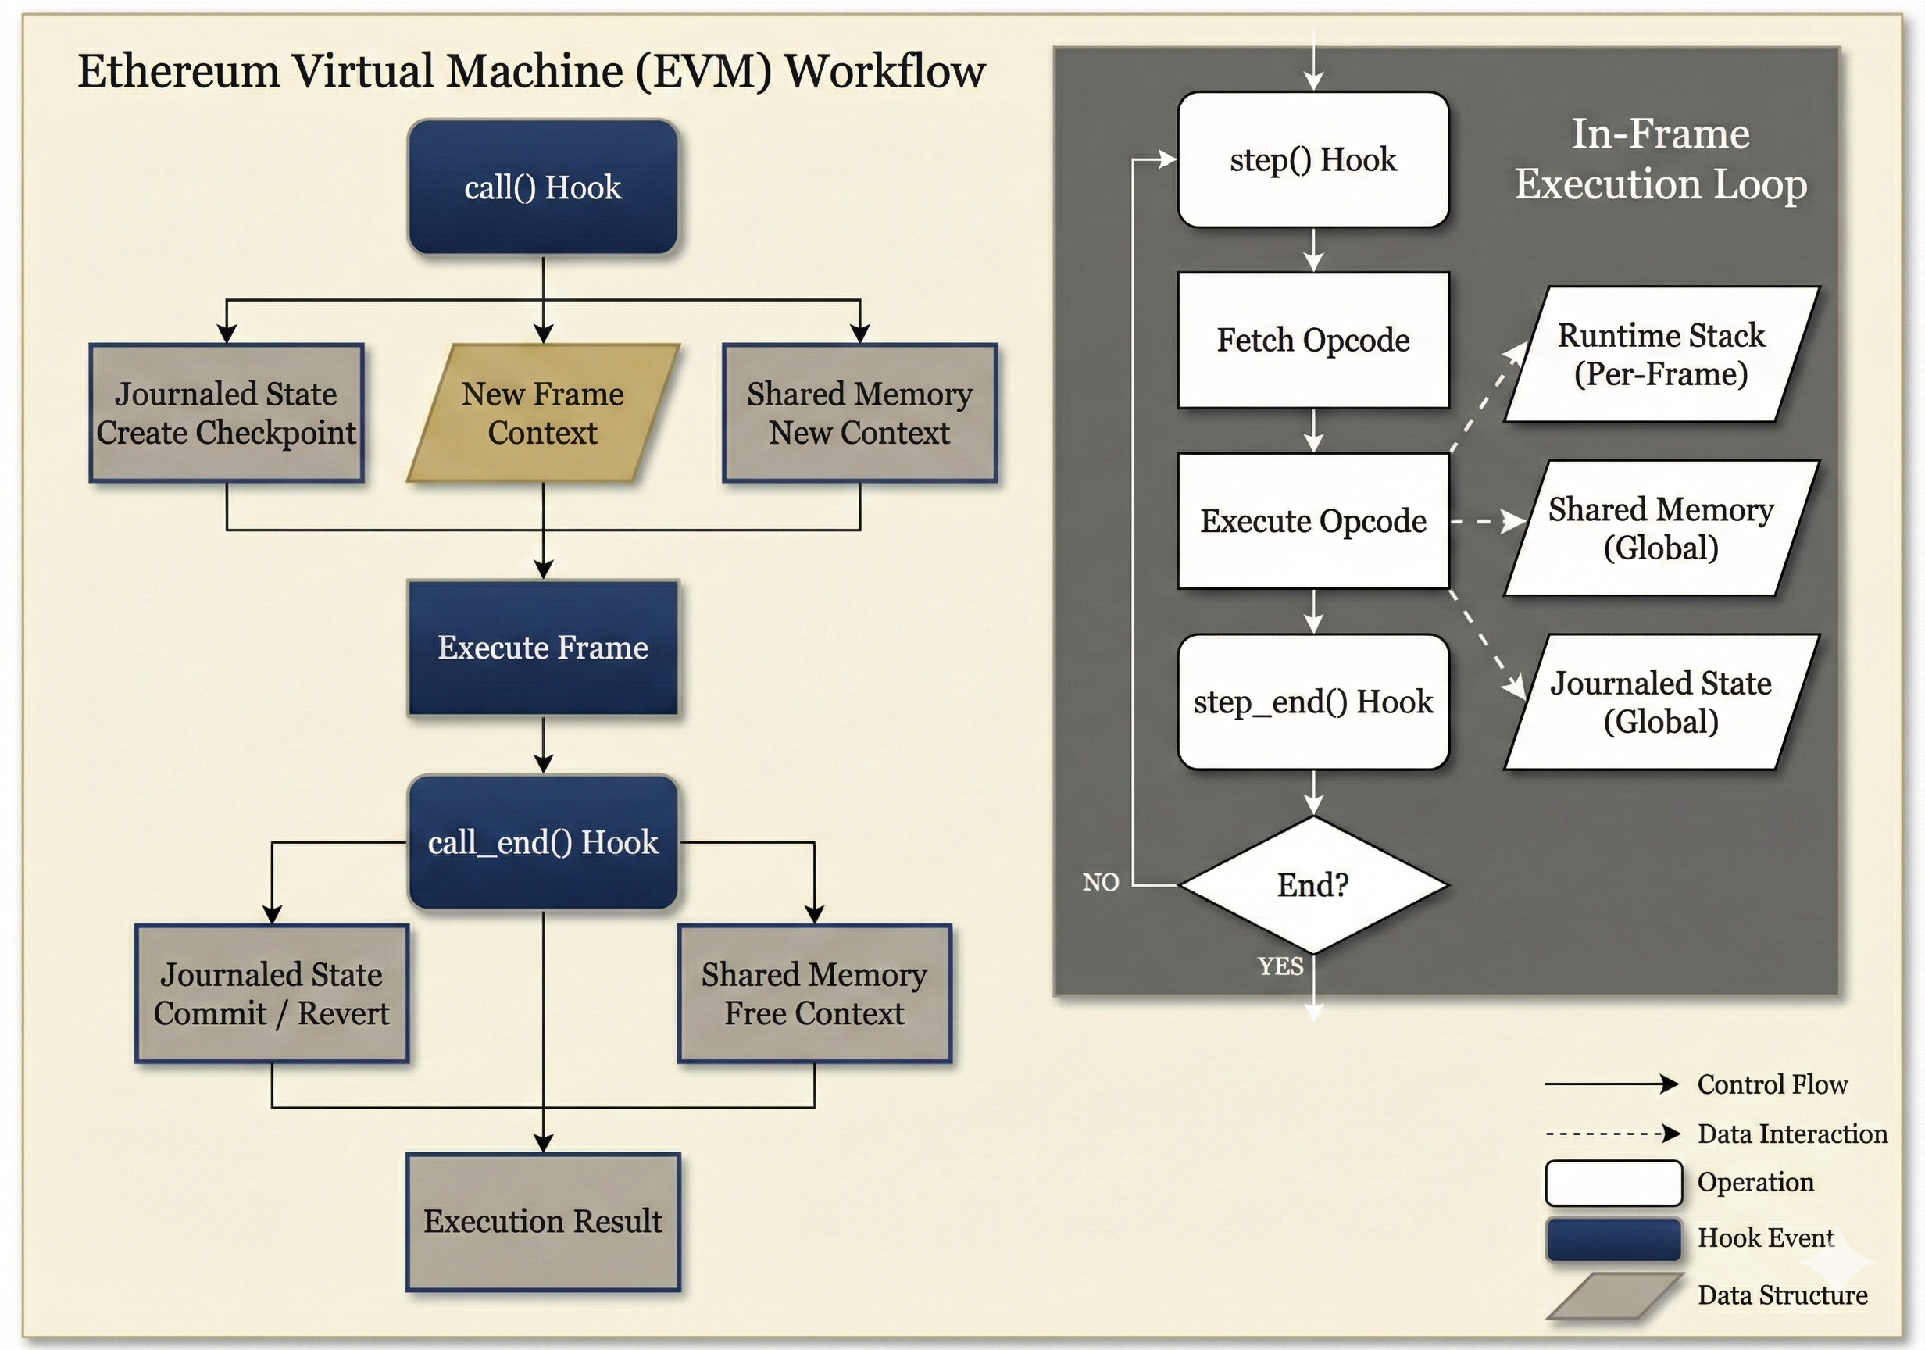
\includegraphics[width=\columnwidth]{raw-figures/EVM.drawio.pdf}
\caption{The EVM execution workflow. The process is partitioned into a high-level frame management lifecycle (left) and a low-level, per-opcode execution loop (right).}
\label{fig:evm-workflow}
\end{figure}


\subsection{The Ethereum Virtual Machine (EVM) Execution Model}
The EVM is a quasi-Turing-complete, stack-based virtual machine that serves as the sandboxed execution environment for smart contracts on the Ethereum blockchain. Its architecture and state model impose specific constraints and present unique opportunities for optimization, which directly inform the design of Helios. The overall execution workflow, depicted in Figure~\ref{fig:evm-workflow}, is partitioned into a high-level frame management lifecycle and a low-level, per-opcode execution loop. The following subsections detail the key components of this model.

\subsubsection{Stack-Based Architecture}
The EVM operates on a shared, 1024-element deep runtime stack where each element is a 256-bit word. All computational opcodes retrieve their operands by popping from the top of the stack and push their results back onto it. This model contrasts with traditional register-based architectures that operate on named registers via direct addressing. While conceptually simple, the stack-based design necessitates a high frequency of explicit stack manipulation instructions to manage data flow. These instructions, alongside the overhead of indirect memory access through a stack pointer, represent a primary target for optimization in Helios.

As illustrated in the in-frame execution loop of Figure~\ref{fig:evm-workflow}, every operation interacts with this per-frame runtime stack. Stack manipulation instructions, such as DUP1-DUP16 for duplicating items at various depths and SWAP1-SWAP16 for swapping the top element with items at different positions, are prevalent in EVM bytecode as compiler-generated boilerplate for managing operand placement. Unlike computational opcodes, these instructions rearrange existing stack elements without producing new values, making them particularly amenable to elimination.

\subsubsection{State Model: Volatile Memory and Persistent Storage}
The EVM maintains two distinct data storage mechanisms: transient memory and persistent storage, visually represented in Figure~\ref{fig:evm-workflow} as Shared Memory and Journaled State respectively. Memory is a byte-addressable linear array with transaction-scoped lifetime, utilized for ephemeral data such as function call arguments and intermediate computation buffers. Storage, by contrast, implements a persistent key-value mapping from 256-bit keys to 256-bit values, constituting the contract's global state that persists across transaction boundaries. Operations on storage are computationally more expensive than memory operations due to their impact on the global state.

The modification of memory and storage constitutes an observable side effect. This characteristic constrains compiler optimizations, as operations with such side effects cannot be reordered or eliminated without altering program semantics. Consequently, Helios focuses its most aggressive optimizations on the computational, side-effect-free operations that occur between state interactions.

\subsubsection{Call Frames}
EVM execution is organized into a hierarchy of call frames. The lifecycle of a single frame, from its creation to its finalization, is depicted in the workflow on the left side of Figure~\ref{fig:evm-workflow}. A new frame, with its own independent memory and runtime stack, is created for each function call, including external calls between different smart contracts. All frames within a single transaction, however, share access to the same persistent storage. A transaction's execution can thus be modeled as an ordered sequence of these call frames. 

\subsubsection{Hook Mechanism}
The EVM specification includes a standard hook mechanism to support native tracers and debuggers. This interface allows an external component to subscribe to events that are triggered immediately before and after the execution of each opcode, as well as at the entry and exit points of every call frame, which are explicitly marked as Hook Events in Figure~\ref{fig:evm-workflow}. This standard, non-invasive interface is foundational for any external profiling tool, as it enables the passive observation of an execution without modifying the core EVM interpreter.

\subsection{Gas: The Resource Metering Mechanism}
\label{sec:gas}
Gas is the fundamental mechanism in the EVM for metering computational resource consumption. It serves both to incentivize validators for the computational work they perform and to protect the network from denial-of-service attacks by ensuring that all executed operations are paid for.

Every transaction submitted to the network must specify a gas limit, representing the maximum amount of gas the originator is willing to consume. Each opcode executed by the EVM deducts a specific amount of gas from this limit. If the total gas consumed exceeds the limit at any point, the execution is halted, an out-of-gas (OOG) exception is raised, and all state changes made by the transaction are reverted. This mechanism ensures that even programs with infinite loops will eventually terminate, making the otherwise Turing-complete EVM a quasi-Turing-complete machine.

EVM gas costs can be categorized into two types: static and dynamic. Static costs are fixed, compile-time determinable values. The majority of opcodes, such as those for arithmetic or logical operations, have a low, constant gas cost. Dynamic costs are values that depend on the runtime state of the EVM. Examples include the cost of expanding memory, which is a quadratic function of the current memory size, or the cost of an SSTORE operation, which depends on whether a storage slot is being accessed for the first time in the transaction or has been accessed before.

This distinction is central to performance optimization, as it creates the opportunity to aggregate and pre-calculate the cumulative static gas costs of long instruction sequences. Dynamic costs, in contrast, must be calculated at runtime to ensure semantic equivalence.

Certain opcodes, termed gas delimiters, explicitly interact with the gas counter. On healthy execution paths where no out-of-gas exception occurs, these delimiters represent the only points where the gas balance must be observable. GAS reads the current gas balance onto the stack; RETURN, STOP, and REVERT finalize frame execution and require gas verification; CREATE and CREATE2 allocate gas to child contracts. These delimiters partition execution into segments, enabling bulk gas deduction for intervening operations.

\subsection{Node Types of the Ethereum Network}
The dual-mode design of Helios is a direct response to the distinct operational requirements and workload characteristics of the two primary types of nodes in the Ethereum network: Full Nodes and Archive Nodes.

A full node is responsible for participating in the real-time operation of the network. Its primary tasks include receiving new transactions from the peer-to-peer network, executing and validating them, and including them in new blocks. This workload is latency-sensitive, as block production times are fixed. Furthermore, full nodes must process transactions with limited predictability, as they frequently encounter novel smart contracts and previously unseen execution paths. This environment, characterized by low latency requirements and high uncertainty, motivates the need for an execution strategy that can perform on-demand, adaptive optimization as new transactions are observed.

An archive node stores the complete history of the blockchain's state from the genesis block to the present. Its primary workload involves serving historical data queries and, crucially, re-executing large batches of historical blocks, for instance, to sync a new node or for data analysis purposes. This workload is throughput-sensitive, prioritizing the total time to process millions of known, historical transactions over the latency of any single one. The execution is entirely deterministic, as the inputs and outcomes of all historical transactions are already recorded on the blockchain. This high-throughput, deterministic workload motivates the need for a specialized execution strategy that can leverage pre-computed knowledge of historical executions to achieve maximum speed with zero speculation overhead.

\subsection{Foundational Concepts in Code Optimization}
The design of Helios's SSA Optimizer is informed by foundational concepts from the field of compiler theory. A key concept is Static Single Assignment (SSA), an intermediate representation property where each variable is assigned a value exactly once. This property makes data dependencies explicit and simplifies a wide range of optimizations. An execution trace that assigns a unique identifier (e.g., a sequence number) to the result of every operation naturally produces an SSA-like representation. Additionally, the EVM ecosystem presents a clear opportunity for a caching system to implement a code/data separation strategy. Contract standards like ERC-20 result in thousands of deployed instances that share identical logic but differ only in their initial constant values, such as a token's name or total supply. With this background on the EVM's architecture, its resource metering model, and the operational context of blockchain nodes, we now proceed to motivate the design of Helios, addressing the limitations of existing approaches.

\subsection{Prior EVM Optimization Approaches}
Recent systems have explored path-driven optimization strategies to accelerate EVM execution. Forerunner~\cite{forerunner} employs constraint-based speculative execution, pre-executing transactions in the transaction pool and generating optimized fast-path programs guarded by control-flow and data-dependency constraints. Seer~\cite{seer} introduces fine-grained branch prediction with checkpoint-based snapshots to maximize pre-execution result reuse across different execution paths. ParallelEVM~\cite{parallelEvm} achieves operation-level concurrent transaction execution through SSA-based conflict detection and selective re-execution of conflicting operations. EVMTracer~\cite{evmTracer} provides dynamic analysis tools to construct opcode-level dependency graphs for quantifying parallelization potential and computational redundancy.

These systems employ comprehensive tracing mechanisms that capture complete execution state, including stack operations, memory accesses, and storage dependencies, enabling detailed analysis and optimization of execution paths across EVM-compatible blockchain systems.